\section{Billboards}
\label{sec:vis_billboards}
We could in principle create a spherical shape by connecting triangles and/or other primitives as illustrated in figure \ref{fig:visualization_glut_spheres}. The figure contains two spheres with different numbers of primitives. We need a substantial number of primitives to get a shape that looks like a sphere (200 in the left sphere in the figure), but we can cheat a bit, by instead rendering something that \textit{looks} like a sphere
\begin{figure}[h]
\begin{center}
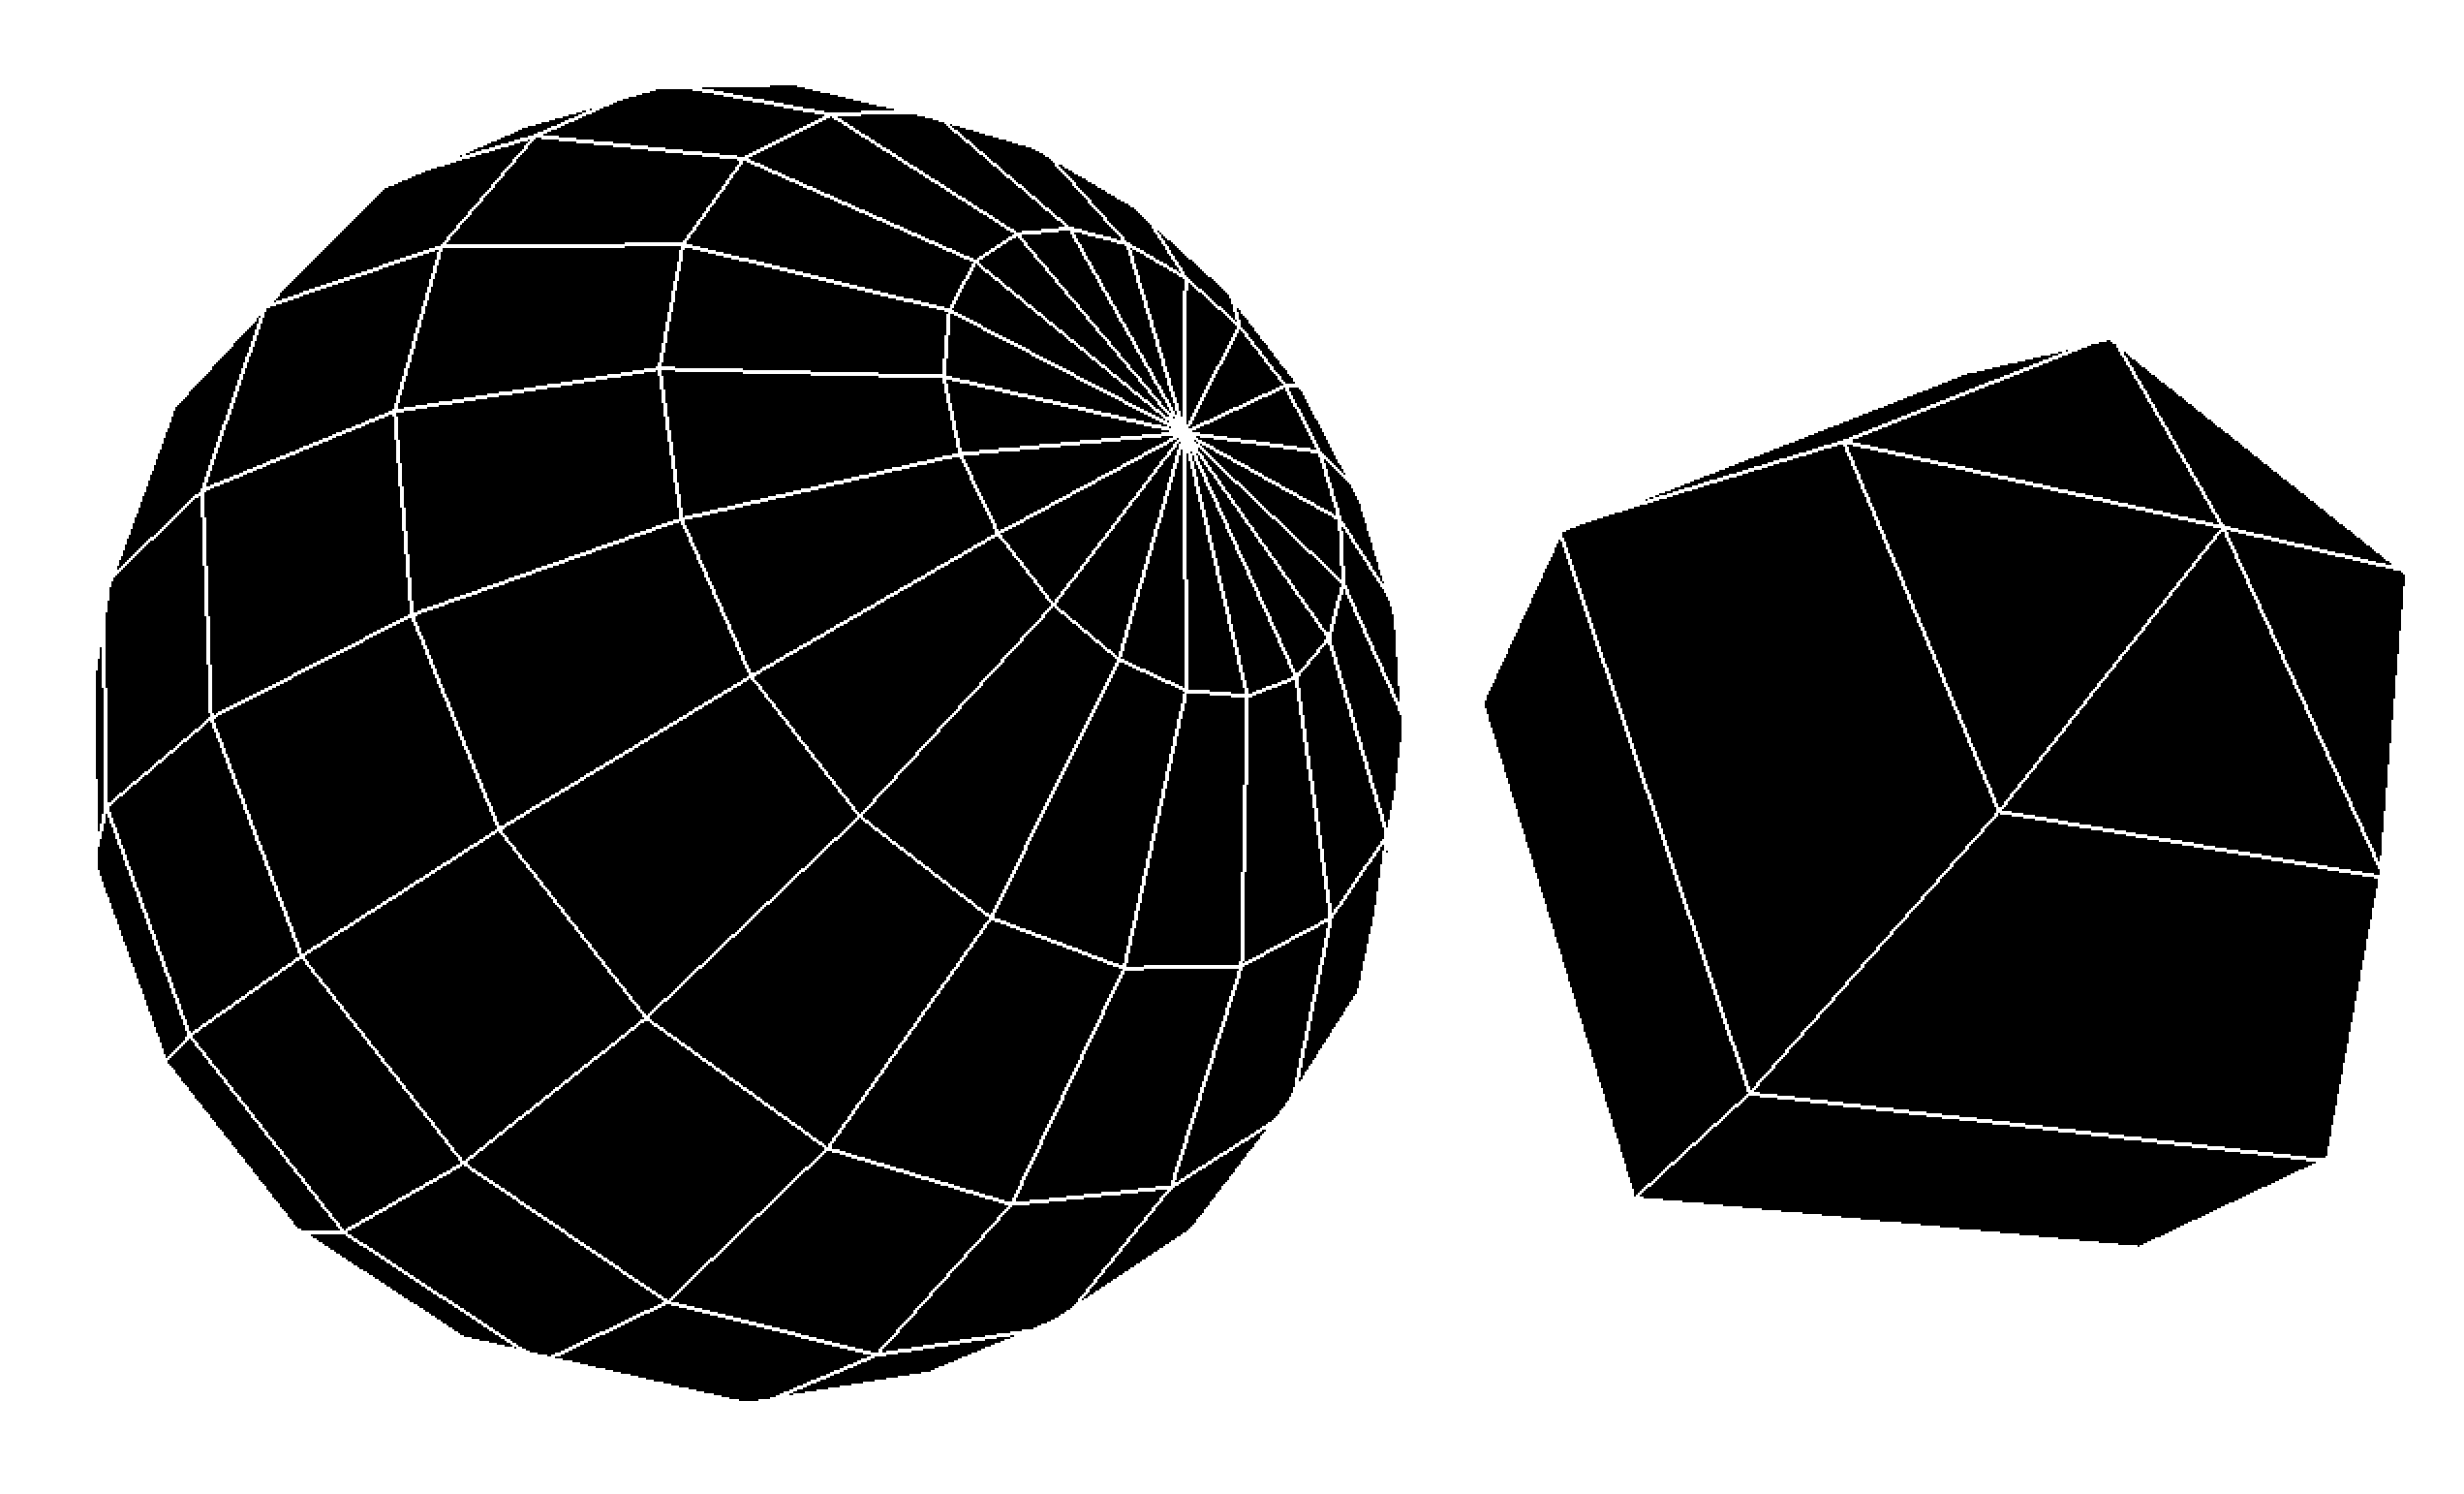
\includegraphics[width=0.8\textwidth, trim=0cm 0cm 0cm 0cm, clip]{visualization/figures/glut_spheres.png}
\end{center}
\caption{A sphere can be created by connecting triangles and/or other primitives. The sphere to the left is made of 200 primitives whereas the one to the right is made of 25 primitives. It is clear that we need a certain number, more than 25, of primitives before we are convinced that the object should represent a sphere.}
\label{fig:visualization_glut_spheres}
\end{figure}
A billboard is, as the name suggests, a rectangle filled with a texture, always pointing towards the camera. The texture is going to be a circle (a sphere does indeed look like a circle when rendered on the screen anyway). It is quite easy to render such a rectangle with OpenGL, we already have a primitive called \textit{GL\_QUADS} which is exactly what we need. The only thing we need to do is provide four vertices, the corners in the rectangle, and give each vertex a texture coordinate. The four vertices $\vec v_i$ can be calculated from one single vertex $\vec r$, the particle position, by
\begin{align}
	\label{eq:vis_vertices_billboard}
	\vec v_1 &= \vec r + (-\Delta x, -\Delta y)\\
	\nonumber
	\vec v_2 &= \vec r + (-\Delta x, \Delta y)\\
	\nonumber
	\vec v_3 &= \vec r + (\Delta x, \Delta y)\\
	\nonumber
	\vec v_4 &= \vec r + (\Delta x, -\Delta y),
\end{align}
where ($L_x = 2\Delta x, L_y = 2\Delta y$) is the size of the billboard, see figure \ref{fig:visualization_billboard_vertices}.
\begin{figure}[h]
\begin{center}
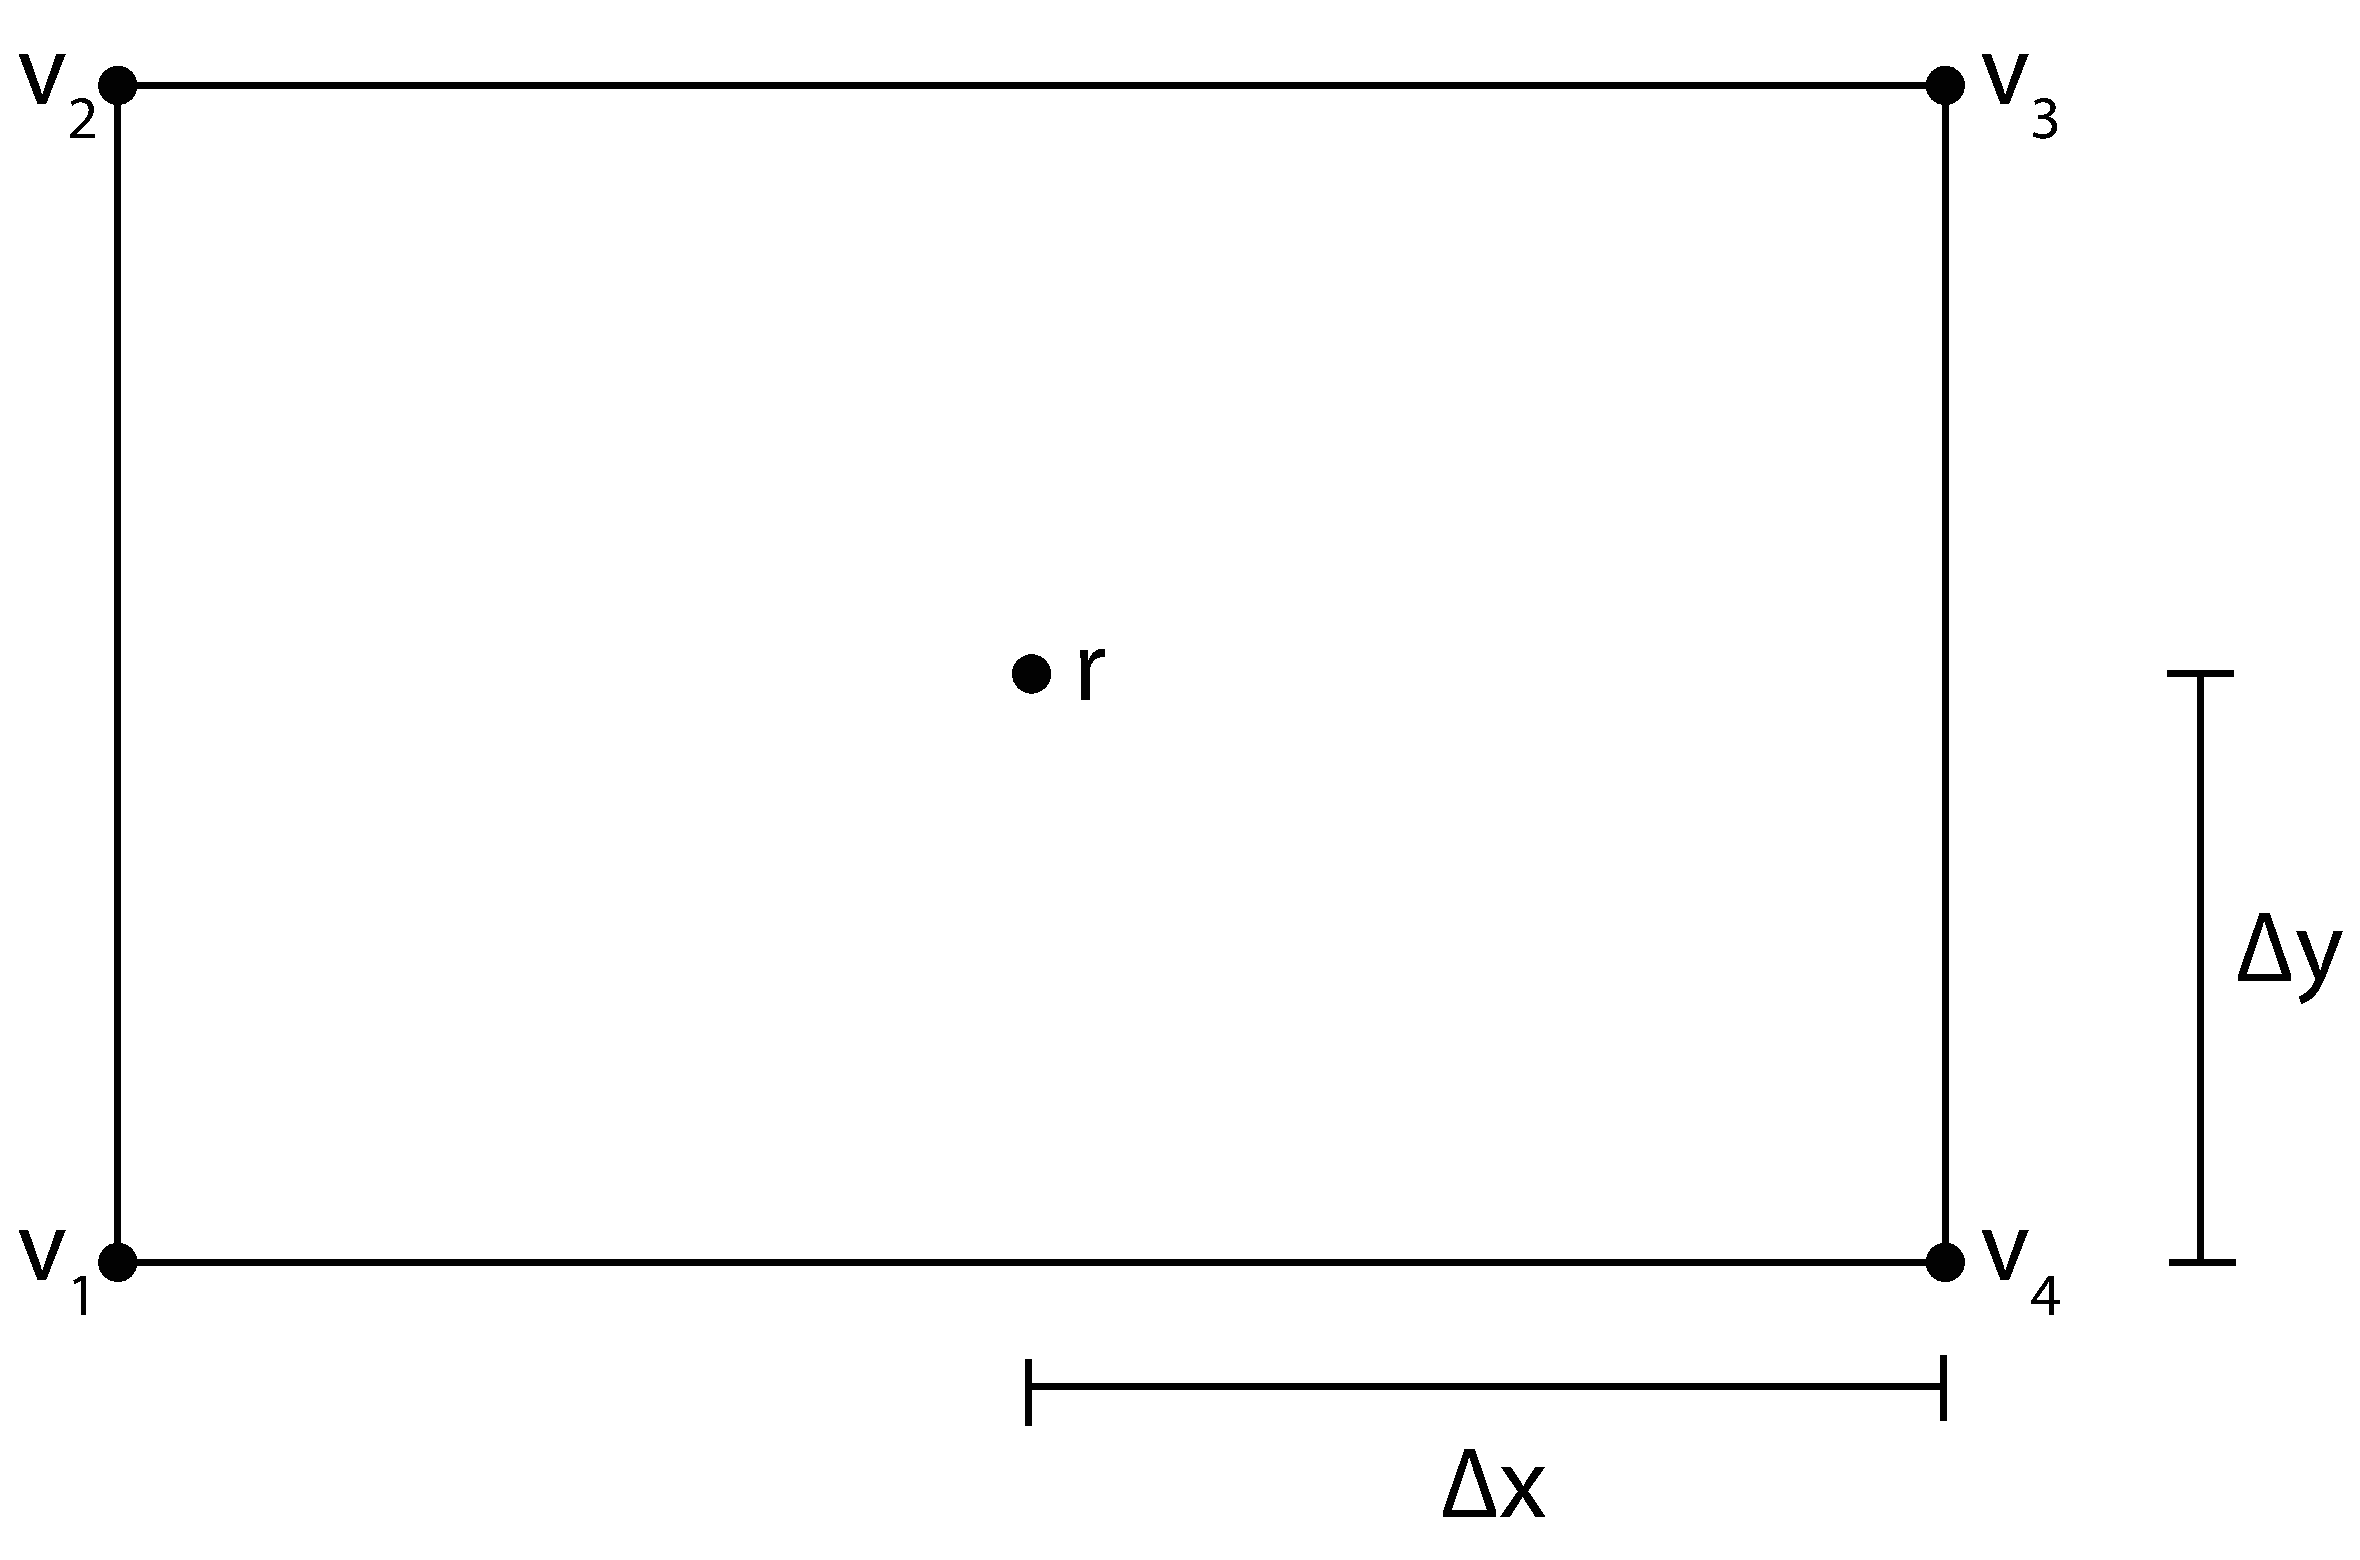
\includegraphics[width=0.7\textwidth, trim=0cm 0cm 0cm 0cm, clip]{visualization/figures/billboard.eps}
\end{center}
\caption{A billboard is made of four vertices $\vec v_1, \vec v_2, \vec v_3$ and $\vec v_4$ that can be calculated from one vertex $\vec r$ (equation \eqref{eq:vis_vertices_billboard}).}
\label{fig:visualization_billboard_vertices}
\end{figure}
This is already what Ovito does\footnote{See the source code at \url{http://www.ovito.org/index.php/download2}}, but we are going to improve this even more. Instead of computing the four vertices and uploading these as \textit{GL\_QUADS} to the GPU, we will only upload the positions of the particles, and exploit the geometry shader to create the billboard vertices on the GPU.\\
Before we start visualizing the data, all timesteps of a simulation are uploaded as VBO's on the GPU so that we don't need to upload data every frame. The VBO is rendered as \textit{GL\_POINTS} so each vertex represents the center position of a particle. We will now follow a single vertex through the pipeline
\subsection{The pipeline}
The VBO can now be seen as one OpenGL model containing the positions of all the particles. The vertices are then in the \textit{model space}. Every single vertex starts its life in the pipeline by going into the vertex shader. The vertex shader is pretty simple in this case, it just transforms the input vertex from the model space to the projection space as we can see in listing \ref{lst:simplevertexshaderbillboard}.
\begin{lstlisting}[caption=billboard\_vertex\_shader.glsl, label=lst:simplevertexshaderbillboard, 
#version 330\n"
uniform mat4 qt_ModelViewProjectionMatrix;
in vec4 qt_Vertex;
void main(void)
{
    gl_Position = qt_ModelViewProjectionMatrix * qt_Vertex;
}
\end{lstlisting}
This position is then sent to the geometry shader as an instance of the \textit{GL\_POINTS} primitive. The geometry shader will, from that single vertex (the position, now in the projection space), create and emit \textit{four} vertices that are displaced from the input vertex as explained in equation \eqref{eq:vis_vertices_billboard} and figure \ref{fig:visualization_billboard_vertices}. The size of the billboard is available as a uniform variable (as explained in subsection \ref{sec:opengl_uniforms}) in the geometry shader. If we want to visualize particles with different sizes (e.g. two atom types with different atomic radii), we just render different VBO's with the corresponding size. We want the four vertices to form a rectangle pointing towards the camera, so the operation in equation \eqref{eq:vis_vertices_billboard} should be done in the view space (here the $z$-direction is orthogonal on the camera plane which forms the $xy$-plane). Since the position vertex now is in the projection space, we should transform the four displacement vectors to the projection space by applying the \textit{qt_ProjectionMatrix} before we add them together. We then set the texture coordinate (the local coordinate in the texture image) on each vertex and emit it with the \textit{EmitVertex()} function. The algorithm might be easier to understand with a code example, see listing \ref{lst:simplegeometryshaderbillboard}.
\begin{lstlisting}[caption=billboard\_geometry\_shader.glsl, label=lst:simplegeometryshaderbillboard, language=GLSL]
#version 400
layout( points ) in;
layout( triangle_strip, max_vertices = 4 ) out;
uniform mat4 qt_ProjectionMatrix;
uniform vec2 size;
out vec2 texCoord;

void main(void) {
    vec4 pos = gl_in[0].gl_Position;
    gl_Position = pos + qt_ProjectionMatrix*vec4(-size.x, -size.y, 0.0, 0.0);
    texCoord = vec2(0.0, 0.0);
    EmitVertex();
    gl_Position = pos + qt_ProjectionMatrix*vec4(-size.x, size.y, 0.0, 0.0);
    texCoord = vec2(0.0, 1.0);
    EmitVertex();
    gl_Position = pos + qt_ProjectionMatrix*vec4(size.x, -size.y, 0.0, 0.0);
    texCoord = vec2(1.0, 0.0);
    EmitVertex();
    gl_Position = pos + qt_ProjectionMatrix*vec4(size.x, size.y, 0.0, 0.0);
    texCoord = vec2(1.0, 1.0);
    EmitVertex();
    EndPrimitive();
}
\end{lstlisting}
This is done with every single position vertex in the VBO (once per particle per frame) and all the output primitives from the geometry shader will be rasterized, clipped and texture coordinates are interpolated into the fragment shader that is run once per pixel per visible primitive. Before we discuss the fragment shader, we should take a look at the texture that each billboard will have.\\
We didn't lie before, we will use a circle that actually is a real sphere rendered in the 3D modeling program Blender\footnote{See \url{http://www.blender.org/} for details}. With some lighting, we get this nice shiny effect making the \"spheres\" look more interesting. This texture is shown in figure \ref{fig:visualization_billboard_texture}, where we also see that all the pixels outside the circles are transparent. This is very important so that we can discard these contributions in the fragment shader.
\begin{figure}[h]
\begin{center}
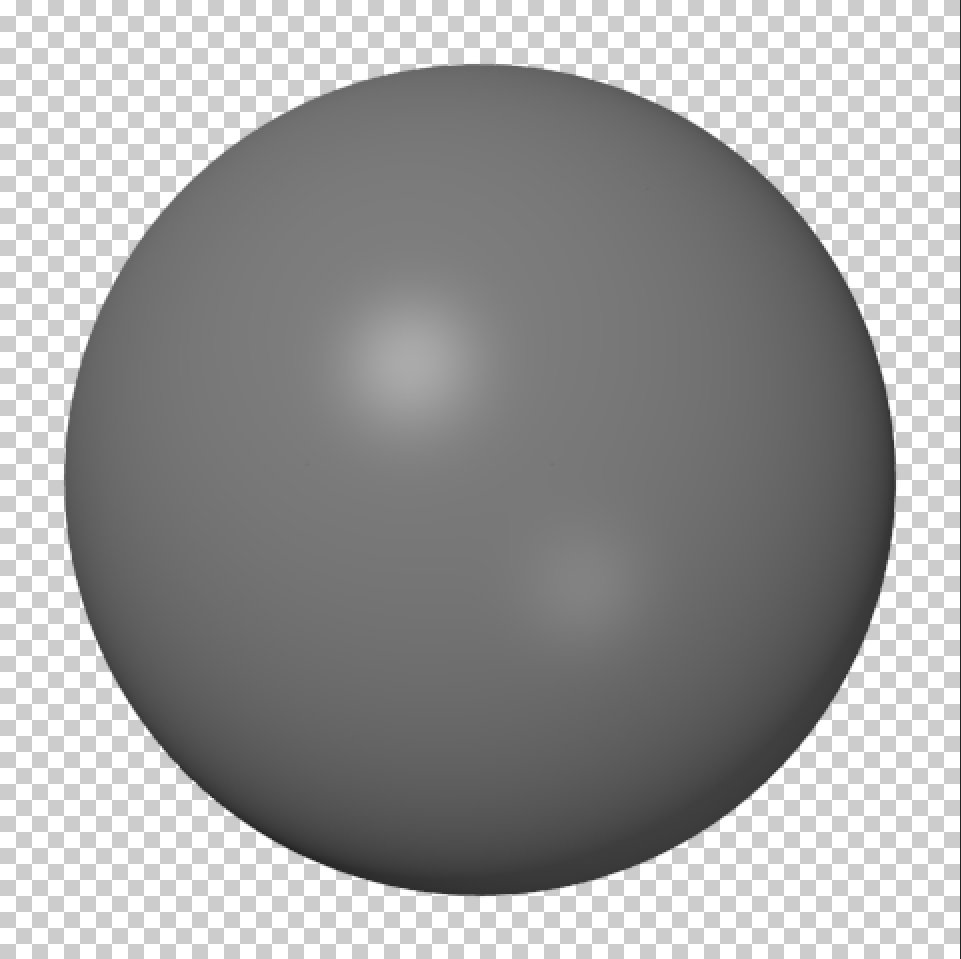
\includegraphics[width=0.7\textwidth, trim=0cm 0cm 0cm 0cm, clip]{visualization/figures/texture_transparent.png}
\end{center}
\caption{The texture used on the billboards is a circle which is a real sphere rendered with Blender. Notice that the pixels outside the circle are transparent. This allows us to discard these texture pixels in the fragment shader.}
\label{fig:visualization_billboard_texture}
\end{figure}
The fragment shader will then get an interpolated texture coordinate as input which we will use to look up which value this pixel gets from the texture. Now is the time for another detail, the color of the particles. Again we assume that all particles have the same color, so as the size variable, it is available as a uniform variable. The final pixel color is then found by equation \eqref{eq:opengl_combining_colors_textures}
\begin{align}
	\vec C(\vec p) = \vec c_t[\vec t(\vec p)] \odot \vec c(\vec p).
\end{align}
The fragment shader code is shown in listing \ref{lst:simplefragmentshaderbillboard} with the final rendering result in figure \ref{fig:visualization_billboard_md}. In this rendered image, we also added light effects making atoms that are far away from the camera appear darker. This increases the feeling of depth which clarifies the pore structures.
\begin{lstlisting}[caption=billboard\_fragment\_shader.glsl, label=lst:simplefragmentshaderbillboard, language=GLSL]
#version 330
uniform vec4 color;
uniform sampler2D qt_Texture0;
in vec2 texCoord;
out vec4 MyFragColor;

void main(void) {
    MyFragColor  = texture2D(qt_Texture0, texCoord.st);
    MyFragColor  = MyFragColor * color;
    if(MyFragColor.a < 0.9999) {
        discard;
    }
}

\end{lstlisting}

\begin{figure}[h]
\begin{center}
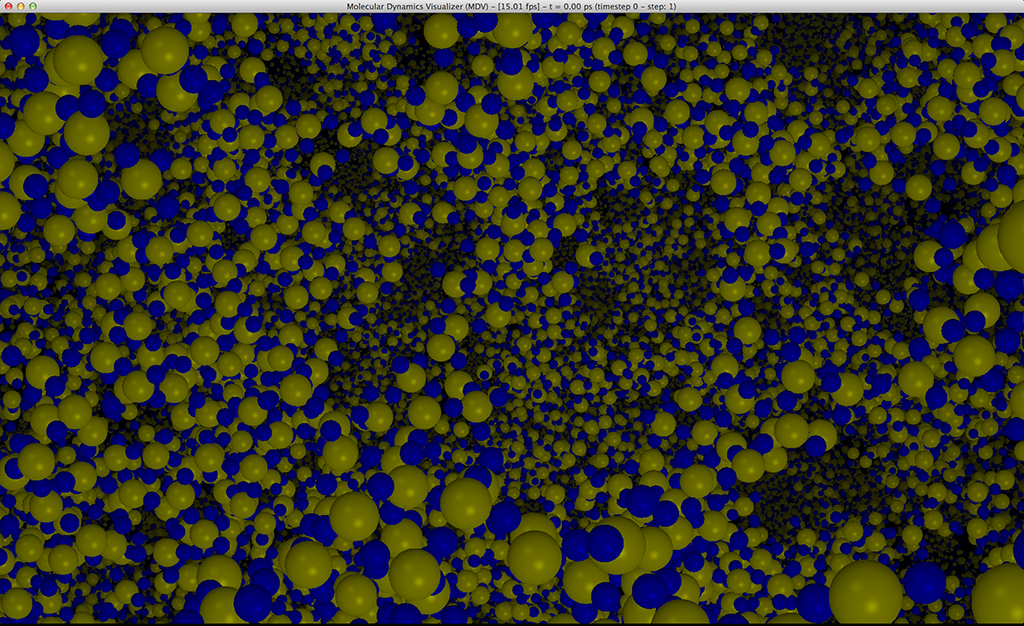
\includegraphics[width=\textwidth, trim=0cm 0cm 0cm 0cm, clip]{visualization/figures/billboards_md_visualization.png}
\end{center}
\caption{The final rendering result with an MD simulation using billboards. In the rendering, light effects are added to increase the depth feeling clarifying the pore structure. This system is a nanoporous SiO2 system simulated with the REMD22 code developed at USC.}
\label{fig:visualization_billboard_md}
\end{figure}

\subsection{Periodic copies}
